\documentclass[12pt]{amsart}
\usepackage{amsmath,amsthm,amssymb,amsfonts,enumerate,mymath,tikz-cd,fancyhdr}
\openup 5pt
\author{Blake Farman\\University of South Carolina}
\title{Math 116\\Homework 09}
\date{December 1, 2015}
\pdfpagewidth 8.5in
\pdfpageheight 11in
\usepackage[margin=1in]{geometry}

\theoremstyle{plain}
\newtheorem{thm}{}
\renewcommand{\qedsymbol}{}

\begin{document}
\maketitle

\section*{14.3}
\renewcommand{\exp}[1]{\operatorname{e}^{#1}}
Consider the following triangle.\\
\begin{center}
  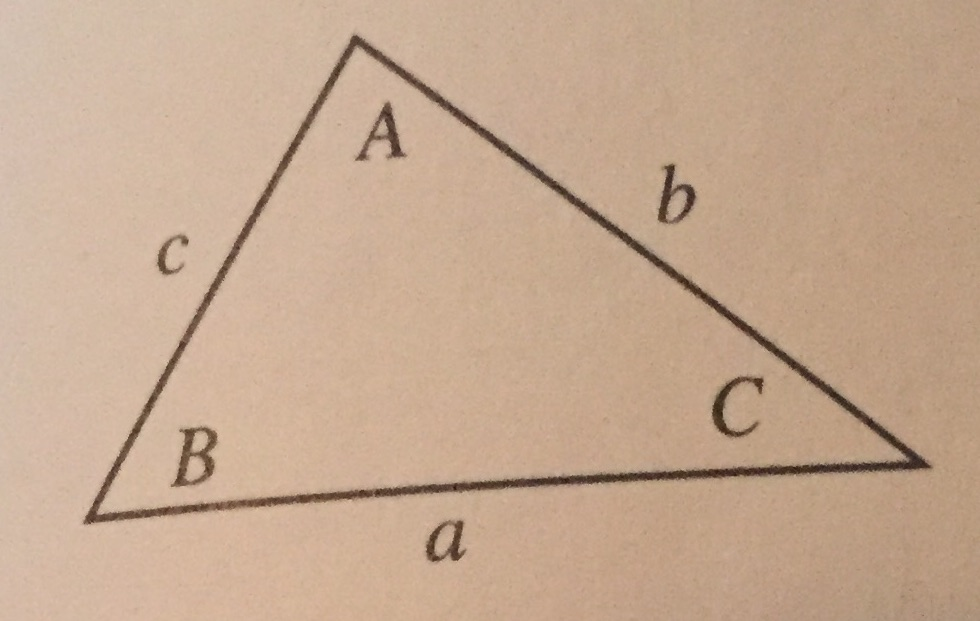
\includegraphics[scale=0.25]{triangle.jpg}
\end{center}
\setcounter{thm}{1}
\begin{thm}
  If $a = 6$, $b = 5$, and $C = 60^\circ$, solve the triangle.
\end{thm}

\setcounter{thm}{3}
\begin{thm}
  Let $C = 20^\circ$, $c = 2$, and $b = 5$.
  Find two triangles with these measures.
  Draw the triangles.
\end{thm}

\newpage
\section*{15.1}

\setcounter{thm}{1}
\begin{thm}
  Write $\cos^5(x)$ as $cos(x) \cdot (\text{some function of}\ \sin(x))$
\end{thm}

\setcounter{thm}{3}
\begin{thm}
  Write $\sec^7(x)$ as $\sec^2(x) \cdot (\text{some function of}\ \tan(x))$.
\end{thm}

\setcounter{thm}{5}
\begin{thm}
  Calculate $\cos(120^\circ)$ and $\sin(15^\circ)$ using the sum and/or difference formulas.
\end{thm}
\end{document}
